\documentclass[twoside]{report}
\usepackage[utf8]{inputenc}
\usepackage[spanish]{babel}
\usepackage{amsmath}
\usepackage{amsfonts}
\usepackage{booktabs}
\usepackage{amssymb}
\usepackage{makecell}
\usepackage{lipsum}
\usepackage{float}
\usepackage{url}
\usepackage{eurosym}
\usepackage[table,xcdraw]{xcolor}
\setcounter{secnumdepth}{3}
\usepackage{multirow}
\usepackage{multicol}
\usepackage{cite}
\usepackage{layout}
\renewcommand{\baselinestretch}{1.2}
\setlength{\parindent}{1cm}
\usepackage{helvet}
\usepackage{graphicx}
\renewcommand{\familydefault}{\sfdefault}

\addto\captionsspanish{\renewcommand{\bibname}{}}
\addto\captionsspanish{\renewcommand{\contentsname}{Índice de contenidos}}
\addto\captionsspanish{\renewcommand{\listfigurename}{Índice de figuras}}
\addto\captionsspanish{\renewcommand{\listtablename}{Índice de tablas}}

\usepackage{geometry}
\geometry{showframe=false,a4paper,left=2cm, right=1.5cm,top=1.6cm,bottom=1.5cm, includehead,includefoot}
\usepackage{fancyhdr}

\fancyhf{}
\renewcommand\headrulewidth{0pt}
\fancyhead[CO,CE]{\begin{small}Route66App: Aplicación móvil de gamificación empresarial para conseguir fidelización de cliente	\end{small}\\\hrulefill}
\fancyfoot[RO, LE]{\hrulefill\\\thepage}

\fancypagestyle{plain}{%
  \fancyhf{}
  \fancyhead[CO,CE]{\begin{small}Route66App: Aplicación móvil de gamificación empresarial para conseguir fidelización de cliente	\end{small}\\\hrulefill}
  \fancyfoot[RO, LE]{\hrulefill\\\thepage}
}


\pagestyle{fancy}

%%%%%%%%%%%%%%%%%%%%%%%%%%%%%%%%%%%%%%%%%%%%%USER CASE COMMANDS

\usepackage{booktabs}

\newcommand\addrow[2]{#1 &#2\\ }

\newcommand\addheading[2]{#1 &#2\\ \hline}
\newcommand\tabularhead{\begin{tabular}{lp{0.7\textwidth}}
\hline
}

\newcommand\addmulrow[2]{ \begin{minipage}[t][][t]{2.5cm}#1\end{minipage}% 
   &\begin{minipage}[t][][t]{8cm}
    \begin{enumerate} #2   \end{enumerate}
    \end{minipage}\\ }

\newenvironment{usecase}{\tabularhead}
{\hline\end{tabular}}

%%%%%%%%%%%%%%%%%%%%%%%%%%%%%%%%%%%%%%%%%%%%%%%%%%%%%%%%%%%%

%%%%%%%%%%%%%%%%%%%%%%%%%%%%%%%%%%%%%%%%%%%%%RISK MANAGEMENT

\newenvironment{risk}{\tabularhead}
{\hline\end{tabular}}

%%%%%%%%%%%%%%%%%%%%%%%%%%%%%%%%%%%%%%%%%%%%%%%%%%%%%%%%%%%%

%%%%%%%%%%%%%%%%%%%%%%%%%%%%%%%%%%%%%%%%%%%%%REQUERIMENT

\newenvironment{req}{\tabularhead}
{\hline\end{tabular}}

%%%%%%%%%%%%%%%%%%%%%%%%%%%%%%%%%%%%%%%%%%%%%%%%%%%%%%%%%%%%




\author{Álvaro Carreras Regorigo}
\title{Route 66}
\begin{document}
\pagenumbering{gobble}
\begin{titlepage}
\begin{center}

\includegraphics[scale=0.5]{images/logoUVa}\\\vspace{1cm}
\begin{LARGE}\textbf{Universidad de Valladolid}\end{LARGE}\\
\vspace{2cm}
\begin{Huge}Escuela de Ingeniería Informática\end{Huge} \\\vspace{0.5cm}
\begin{large}\textsc{\textbf{TRABAJO FIN DE GRADO}}\end{large}\\ \vspace{2.5cm}
\begin{Large}Grado en Ingeniería Informática \\ (Mención en Ingeniería de Software)\end{Large}\\ \vspace{4cm}
\begin{Huge}\textbf{Route66App}\end{Huge}
\end{center}\vspace{2cm}
\begin{flushright}
\begin{large}Autor: \\\textbf{D. Álvaro Carreras Regorigo}\\
Tutora:\\
Dña. Margarita Gonzalo Tasis\end{large}
\end{flushright}
\end{titlepage}
\clearpage

\tableofcontents

\listoffigures
 
\listoftables

\clearpage
\pagenumbering{arabic}
\chapter{Parte I: Introducción y contexto.}
\section{Introducción y objetivos.}

\subsection{Introducción.}

La ludificación o gamificación (del inglés, gamification) consiste, según IEBSchool en “el uso de mecánicas de juego en un contexto de no juego para conducir el comportamiento de los participantes (mediante la participación, la interacción, la adicción o, incluso, la competición) hacia la consecución de un determinado objetivo de negocio” \cite{iebschoolGami}. 

Aunque típicamente se ha visto la ludificación aplicada al área comercial o de ventas, existen otros ejemplos en la educación o incluso en las relaciones con los proveedores o para incrementar el número de ventas en un centro comercial (ludificación orientada a los empleados).

Hoy en día, miles de compañías utilizan la ludificación en sus procesos empresariales, desde sus relaciones con los empleados, hasta con los clientes, pasando por sus comerciales. La ludificación realmente funciona y, por increíble que parezca, es muy efectiva.

No son pocos los ejemplos de una aplicación más que satisfactoria de la misma. En 2011, Volskwagen decidió inventar en China, su mercado más importante, una nueva versión de su \textit{people’s car}. Para ello contó con la ayuda de sus clientes, a quienes ofreció una herramienta de diseño y un sistema de puntuaciones. El resultado del mismo fue la obtención de más de 50.000 propuestas diferentes.

Hay otros ejemplos, por ejemplo, Correos decidió en 2012 rediseñar su web y se le plantearon o bien contratar a una empresa por miles de euros, o bien, plantear un sistema de gamificación en el que los empleados propusieran nuevos diseños, a cambio de pequeños regalos. Aplicaron la ludificación y esto supuso un ahorro de un 70\%. Se presentaron más de 50.000 ideas en un tiempo récord de tiempo.

Quizá el caso más destacable en nuestro país es el de BBVA Game\cite{bbvag}, una plataforma de ludificación asociada a la banca virtual. En ella, los usuarios consiguen puntos al superar distintos retos, entre los que se encuentran consultar movimientos, domiciliar la nómina, realizar transferencias... Igualmente, también se pueden conseguir puntos por compartir un mensaje en redes sociales, así como invitar a amigos o contratar productos. Con todos estos puntos, es posible canjearlos por premios directos, o bien, por participaciones en los sorteos que realizan. El resultado de este proyecto fue un éxito rotundo, ya que consiguieron 100.000 nuevos clientes en los nueve primeros meses, así como aumentar el uso de la plataforma que hacian sus clientes ya existentes.

\subsection{Objetivos.}

El objetivo de este Trabajo Fin de Grado es el de realizar una aplicación Android para un restaurante de comida rápida, que cuente con un sistema de ludificación. En concreto, se realizará basándose en la idea desarrollada en el Trabajo de Fin de Grado de Dª Cristina Martínez Martínez\cite{cristinatfg}. Los objetivos concretos de la aplicación vendrán detallados en el documento de análisis.

Este TFG detallará el desarrollo, análisis, diseño e implementación de la parte cliente del sistema informático en cuestión. Se ha diseñado para que este cambie las diferentes misiones y desafíos, de acuerdo con los parámetros que el administrador del sistema establezca en el backend (parte de gestión).

\subsection{Motivación.}

Este trabajo tiene una doble motivación, por un lado, analizar, diseñar e implementar un sistema de ludificación diseñado por una alumna de esta Universidad, para completar así, una de las líneas futuras propuestas por la misma en su Trabajo de Fin de Grado. 

Por otro, se busca desarrollar un sistema de ludificación que permita a los alumnos del Grado en Organización Industrial de nuestra Universidad, poner en marcha y probar un sistema de este tipo, ya que las alternativas existentes en el mercado no ofrecen posibilidad de prueba como estudiante.

\section{Propuesta.}
Este Trabajo de Fin de Grado estará centrado en el TFG “Estudio de gamificación en una empresa para mejorar la fidelización de los clientes”\cite{cristinatfg}, elaborado por Dª Cristina Martínez Martínez, graduada durante el curso 2016-2017 en Ingeniería de Organización Industrial por la Universidad de Valladolid.  

El trabajo de esta alumna, centrado en el diseño de un sistema de gamificación aplicado a un posible caso real (restaurante de comida americana), tenía el problema de la imposibilidad de llevarlo a cabo con herramientas profesionales, debido a su coste y a la falta de disponibilidad de las mismas. Por este motivo, el TFG se tuvo que defender contando solo con una serie de prototipos basados en un sistema web. 

Como la gamificación es un área en investigacion y que ofrece muy buenos resultados, la tutora del TFG propuso a la Comisión de Título la realización de este trabajo. Por otro lado, el resultado del mismo puede servir a alumnos de otras facultades para poder utilizar una herramienta de gamificación real.

\subsection{Resumen de “Estudio de gamificación en una empresa para mejorar la fidelización de los clientes”}

Se propone la realización de un sistema de gamificación para una cadena de restaurantes de comida americana, que cuenta con un conjunto de franquicias repartidas por todo el territorio español. Es una empresa con muy buenos resultados económicos y cuenta con una amplia y sólida base de clientes, que decide elaborar una aplicación que mejore la opinión de los mismos sobre la marca, ya que han llegado críticas sobre el sistema vigente de cupones y descuentos.

Finalmente, el equipo directivo decide encargar una aplicación basada en la ludificación cuyos objetivos son los siguientes:

\begin{enumerate}
\item Aumentar la fidelización de los clientes.
\item Incentivar las ventas.
\item Mejorar la imagen de la marca en redes sociales.
\item Conseguir nuevos clientes.
\item Mejorar la confianza y satisfacción del cliente. 
\end{enumerate}

Se medirá el cumplimiento de los objetivos anteriores mediante el cálculo de una serie de ratios.\\

\textbf{Público objetivo}\\

El público objetivo estará formado por hombres y mujeres, cuyas edades estén comprendidas entre los doce y los cincuenta y cinco años. 
Los conocimientos tecnológicos esperados en este grupo de edad no tienen por que ser altos, ya que se utilizará una aplicación móvil. Se considerará suficiente por tanto, conocimientos básicos en uso de smartphones y de uso de aplicaciones móviles. En el caso en el que nos encontramos la aplicación a desarrollar será Android.

Los potenciales usuarios de la aplicación la utilizarán para conseguir recompensas y descuentos derivados del uso de la misma.

Finalmente, indicar que se clasificará cada jugador en función de sus gustos y comportamientos, siguiendo la teoría de Battle, haciendo así que la experiencia de usuario sea distinta entre usuarios de distinta categoría. En concreto, se realizarán distintos tipos de juegos.\\

\textbf{Roles}\\

Se proponen dos tipos de roles: Administrador y Cliente.

Las funcionalidades que podrá acceder cada tipo de rol vendrán determinadas en un diagrama de casos de uso que se especificará en el apartado correspondiente. \\

\textbf{Descripción del juego}\\

El juego se centra en un mapa de la Ruta66 americana, aprovechando así la temática del restaurante. Se dividirá el camino en once etapas o niveles, correspondientes a las principales ciudades por las que pasa esta vía, y para avanzar, el cliente deberá completar una serie de actividades, que además otorgarán insignias. Cabe destacar que la dificultad de los niveles irá aumentando gradualmente, con el objetivo de no perder la motivación.

\begin{multicols}{4}
\begin{enumerate}
\item Chicago.
\item Springfield.
\item St. Louis.
\item Tulsa.
\item Oklahoma City.
\item Amarillo.
\item Santa Fe.
\item Albuquerque.
\item Flagstaff.
\item Williams.
\item Los Ángeles.
\end{enumerate}
\end{multicols}

Todos los niveles excepto el de Chicago tendrán un planteamiento similar:
\begin{itemize}
\item Nivel 1. Chicago: Compuesto por diez casillas. Se activarán dos por cada actividad completada:
	\begin{itemize}
		\item Configuración del perfil del jugador.
		\item Crear un equipo.
		\item Seguir en redes sociales la página del restaurante.
		\item Puntuar la aplicación en la tienda de aplicaciones.
		\item Comentar la aplicación en la tienda de aplicaciones.
	\end{itemize}
\item Resto de niveles: Consistirán en diez misiones:
	\begin{itemize}
		\item Misiones de nivel social: consistirán en tareas como compartir el progreso, subir una foto hecha en el restaurante a las redes sociales, enviar invitaciones…
		\item Misiones de minijuegos: serán dos casillas y consistirá en jugar a un minijuego, dependiente del perfil de jugador.
		\item Misiones de consumo: el jugador deberá realizar consumiciones en los restaurantes de la cadena. Avanzará más o menos casillas en función del gasto que realice.
		\item Misiones de retos especiales: en días señalados, los jugadores podrán participar en retos creados específicamente para ese día.
	\end{itemize}
\end{itemize}

\textbf{Recompensas}\\

Hay tres tipos de recompensa:
\begin{itemize}
\item Puntos: el usuario obtendrá diez puntos por cada casilla que avance. Similarmente, se agrupará la suma total en tres categorías: consumo, social y competitivo.
\item Insignias: cuando el jugador haya completado un nivel completo obtendrá una insignia (matrícula de la ciudad asociada). Habrá, adicionalmente, otras insignias, entre las que se encuentran la familiar o las de grupo.
\item Premios: los premios serán regalos. Se desbloquearán cuando el usuario haya completado un nivel o haya realizado algún reto especial.
\end{itemize}

\textbf{Perfiles de jugador\cite{iebsctj}}\\ 

Todos los jugadores tendrán asociado un perfil, que se determinará en el registro de usuario:
\begin{itemize}

\item Triunfador: tendrá como objetivo llevar a cabo las misiones y obtener los premios o recompensas.
\item Explorador: son jugadores que les gusta descubrir o aprender cosas nuevas.
\item Socializadores: más que interés en conseguir los logros, buscan aprovecharlos para entablar relaciones sociales.
\item Killers: buscan ser los primeros en el juego. Quieren destacar sobre otros jugadores.

\end{itemize}

\textbf{Grupos}\\

Los jugadores, similarmente, podrán crear el número que quieran de equipos. Participarán con los mismos a la hora de alcanzar las recompensas.

\section{Análisis de aplicaciones similares}

He seleccionado y analizado diversas aplicaciones de restaurantes de comida rápida asentados en España, con el fin de conocer cómo son y si han implementado técnicas de gamificación a las mismas.

He de destacar que \textbf{ninguna} aplicación ha implementado ningún sistema de ludificación.

\subsubsection{McDonald's \cite{mcdo}}

La aplicación móvil McDonalds ofrece un gran número de funcionalidades, entre las que se encuentran un servicio de ofertas , canjeo de cupones, listado de la carta de productos o envío de pedidos a domicilio. 

No tiene un sistema de ludificación implementado, ya que su estrategia se basa en utilizar un sistema por niveles (oro, plata y bronce), en el que cuanto más alto sea, mejores ofertas se pueden encontrar. Para poder subir de nivel, será necesario escanear los tickets de compra y llegar a un mínimo de gasto.

Destacar que durante el tiempo que ha estado instalada ha pedido dar la opinión de la app por correo electrónico, a cambio de obtener un obsequio.

\subsubsection{Burger King \cite{burgerk}}

Al igual que McDonalds,sí se ofrece un sistema de fidelización, llamado "Mis Coronas". Este programa consiste en que cada tres pedidos realizados por medio de la app móvil o el sitio web de Burger King se acumulan coronas. Cada corona se puede cambiar por una hamburguesa gratis. Además, invitan a registrarse en la app, ya que, con el historial de pedidos realizarán ofertas personalizadas al cliente.

Las opciones de esta app están bastante limitadas y en ellas se encuentran conseguir un listado de restaurantes, realizar pedidos a domicilio, ver la carta de productos o visualizar un listado de cupones o promociones.

\subsubsection{KFC \cite{kfcapp}}

La fidelización de clientes se limita a poner ofertas de acuerdo con los gustos del cliente (ya que utiliza el historial de pedidos).

En cuanto a funcionalidad, se limita a poner una carta de productos, un listado de restuarantes y una opción para obtener ofertas.

\subsubsection{VIPS \cite{vipsapp}}

La aplicación de la cadena VIPS es, sin lugar a dudas, la más completa de las analizadas.

Para fidelizar clientes, utiliza el servicio ClubEuroVIPS, en el que ofrece un \textit{cashback} de un 3\%, pudiendo duplicarse bajo ciertas condiciones. Además ofrece un sistema de clasificación de usuarios según su consumo (niveles clásico, oro y platino), en el que, dependiendo del cuál nos escontremos podremos obtener WiFi Premium, bebidas extras u obtener puntos extras.

Paralelamente, la aplicación invita al usuario, con cierta frecuencia a sus lanzamientos o estrenos de nuevos productos. Por ejemplo “\textit{te invitamos a nuestras hamburguesas del Chef o a nuestras nuevas pizzas Chicago Style}” o “\textit{te invitamos a probar nuestras pizzas}”.

Similarmente, se pueden encontrar funcionalidades propias de un restaurante que apuesta por el crecimiento de su app móvil, como son la posibilidad de pagar un pedido con la app móvil, la funcionalidad \textit{Shake-It}, que consiste en realizar tu pedido favorito con solo agitar tu teléfono móvil o la posibilidad de guardar promociones en la aplicación. Además, también permite realizar pedidos online del tipo \textit{take-away}.

\subsubsection{Pans and Company \cite{pansapp}}

Pans \& Company ofrece únicamente una tarjeta de fidelidad, integrada en la misma app. Esta tarjeta básicamente consiste en un código QR que el usuario puede mostrar en caja para acumular puntos que, posteriormente se podrán convertir en dinero. Además, se realizarán ofertas personalizadas.

Sus funcionalidades son las típicas de una aplicación de esta categoría: listado de restaurantes, ofertas y listado de la carta.

\subsubsection{Foster's Hollywood \cite{fostersh}}

El sistema de fidelización de clientes de Foster's Hollywood se basa en un sistema de niveles (blue, silver y gold), en el que cuanto mejor sea el nivel, mayores ventajas tendrá el usuario, entre las que se encuentran un postre de regalo, descuentos de ocio (en empresas asociadas), o incluso, promoción por el cumpleaños. Para poder aumentar de nivel será necesario ir un número de veces a los establecimientos de la cadena. 

Se nos identificará como clientes mediante la tarjeta Foster's Hollywood, que consiste en un código QR localizado en la aplicación y que el cliente simplemente debe enseñar al realizar el pago, con el fin de que la compra quede asociada a su usuario.

Por otra parte, también es posible visualizar la carta del restaurante o ver el listado de restaurantes, así como realizar el pedido online.

\section{Estructura de la memoria}

Este documento está divido en partes y a su vez estas en secciones y subsecciones, abarcando así los distintos documentos recogidos en esta memoria:

\begin{itemize}
\item Parte I. Introducción y Objetivos: incluye una breve explicación de lo que es la gamificación, así como una explicación a alto nivel de la propuesta realizada por la diseñadora del sistema de gamificación sobre el que está basado el proyecto. Finalmente, también contiene un análisis de aplicaciones de restaurantes de comida rápida que operan en España, con el fin de estudiar si estos incluyen o no un sistema de ludificación.

\item Parte II. Herramientas utilizadas y entorno de trabajo: detallaré aquellas herramientas utilizadas en el proyecto, tanto de tipo \textit{hardware} como de tipo \textit{software}. 

\item Parte III. Route66App: es la parte más importante del proyecto, pues incluye la gran mayoría de documentos, como el Plan de Desarrollo de Software, el documento de análisis, el documento de diseño, los prototipos realizados y todos aquellos detalles de la implementación que merece la pena reseñar.

\item Parte IV. Conclusiones y líneas futuras.

\item Referencias.

\item Anexos

\end{itemize}

\chapter{Parte II: Herramientas utilizadas y entorno de trabajo}
\section{Herramientas utilizadas}

Para la elaboración de esta memoria he utilizado las siguientes herramientas:
\begin{itemize}
\item Como editor \LaTeX , Texmaker v. 4.4.1. \footnote{\url{http://www.xm1math.net/texmaker/}}
\item Como sistema de control de versiones, GitHub \footnote{\url{https://www.github.com}}
\item Para tomar notas e ideas, Dropbox Paper \footnote{\url{https://paper.dropbox.com}}
\end{itemize}

Para la elaboración de los prototipos, he utilizado Ionic 3 \footnote{\url{https://ionicframework.com/}}.

Para la elaboración de la aplicación Android, he utilizando Android Studio.

Para el control y seguimiento del proyecto utilizaré la herramienta Zoho Projects \footnote{\url{https://projects.zoho.com/}}.

Finalmente, he empleado Firebase \footnote{\url{https://firebase.google.com/}}
\section{Entorno de trabajo}

La memoria ha sido escrita usando un ordenador portátil que cuenta con las siguientes características:
\begin{itemize}
\item Marca: Lenovo.
\item Modelo: G-50-70.
\item Memoria principal: 4GB.
\item HDD 500 GB.
\item Sistema Operativo: Xubuntu 17.04 LTS 64 bits.
\end{itemize}

En cuanto al servidor utilizado, será el proporcionado por los técnicos de la Escuela de Ingeniería Informática de Valladolid, en concreto:
\begin{itemize}
\item ...
\end{itemize}
\section{Comunicación con el servidor}

\chapter{Parte III: Route66App}
\section{Plan de Desarrollo del Software}
\subsection{Descripción del proyecto}
La ludificación comenzó a popularizarse en 2010\cite{anatfg}. Desde entonces, tal y como he explicado en puntos anteriores de esta memoria, se ha aplicado en numerosas situaciones (educación, ventas, proveedores...). En el caso que nos ocupa, un restaurante de comida americana, no podemos encontrar en España ningún ejemplo de una aplicación similar que aplique la ludificación.

Route66App consiste en una app para dispositivos móviles que aplica las ideas expuestas en el Trabajo Fin de Grado de una alumna del Grado en Organización Industrial \cite{cristinatfg}. Esta aplicación aplicará la teoría Bartle para identificar los diferentes tipos de jugador y buscará fidelizar y comprometer al usuario con los objetivos del negocio, por medio del juego.

Es importante destacar que este trabajo es solo una parte de dos, el cliente. Para un completo funcionamiento se requerirá el gestor web, en el que se podrán añadir y modificar las diferentes misiones que conforman el juego.
 
\subsubsection{Propósito, objetivos y alcance}

El objetivo fundamental de  este trabajo es el de la implementación de un sistema de ludificación, aplicado a un restaurante de comida americana. En concreto se realizará la parte cliente, ejecutada desde terminales móviles con el Sistema Operativo Android.

La aplicación deberá contar con las siguientes funciones:
\begin{itemize}
\item Acciones propias del usuario
	\begin{itemize}
	\item Realizar misiones y juegos, con el fin de conseguir puntos y aumentar el nivel o posición en un ranking.
	\item Modificación del perfil del usuario, permitiendo actualizar el avatar del usuario.
	\item Consulta del historial de logros del usuario.
	\item Consulta de las insignias del usuario.
	\item Consulta del código QR que identifica al usuario de forma única.
	\item Consulta de la posición global del usuario (ranking).
	\end{itemize}
\item Acciones a realizar en grupo.
	\begin{itemize}
	\item Cosulta de los equipos a los que pertenece el usuario.
	\item Creación de nuevos equipos.
	\end{itemize}
\end{itemize}

Los objetivos serán:
\begin{itemize}
	\item Elaborar un sistema de usuarios, mediante el uso de sesiones.
	\item Gestionar un sistema de insignias, otorgadas tanto a usuarios individuales, como a grupos o equipos completos.
	\item Aumentar el \textit{engagement} del usuario con la aplicación, mediante el uso de juegos o misiones.
	\item Hacer las funciones de una tarjeta de fidelización virtual, que permita al usuario identificarse a la hora de pagar.
\end{itemize}

\subsection{Metodología de Desarrollo del proyecto}
El proyecto aplicará el Proceso Unificado (\textit{Unified Process}), en concreto el proceso UPedu \cite{upedu}, cuyas caracterísiticas básicas \cite{pgpup} son: 
\begin{itemize}
\item Dirigido por los casos de uso.
\item Centrado en la arquitectura.
\item Iterativo e incremental
\end{itemize}
La iteratividad supone ciertas ventajas, como que se pueden mitigar los riesgos más críticos en las fases más tempranas o que permite obtener \textit{feedback} mucho antes, además, el aprendizaje obtenido se puede reaprovechar en etapas posteriores.
\subsection{Restricciones}
Se imponen las siguientes restricciones:
\begin{enumerate}
\item \textbf{Tiempo:} Este proyecto se realiza para cumplir con los objetivos de la asignatura Trabajo de Fin de Grado. Mención Ingeniería del Software, correspondiente a 12 créditos ECTS, unas 300 horas.

\item \textbf{Plazo mínimo de entrega:} Este proyecto se podrá entregar cuando haya terminado el resto de asignaturas de la Mención. Por tanto, hasta que no termine y tenga calificada la única asignatura que tendré en el segundo cuatrimestre (Prácticas de Empresa), no podrá ser entregado. Según mi planificación, la práctica comenzará a finales del mes de Enero de 2018 y terminará por Abril.

\item \textbf{Requisitos de la plataforma:} La aplicación será instalable en terminales Android, cuya versión de API sea igual o superior a la 4.4. Según el sitio Web oficial de desarrolladores de Android \footnote{\url{https://developer.android.com/}}, esto supone cubrir la grandísima mayoría de los dispositivos (un 92.5, a fecha 25 de Noviembre de 2017)\cite{androidversiondist}.

\item \textbf{Herramientas:} Se utilizará Firebase \footnote{\url{https://firebase.google.com/?hl=es-419}}. En concreto, las utilidades Analytics, Authentication, Crash Reporting Service, Storage, Notifications y Predictions.

\item \textbf{Persistencia de datos: } Contaré con el servicio de gestión de bases de datos SQLite que ofrece Android de serie, con el fin de reducir la carga de peticiones que haga el usuario contra la plataforma.
\end{enumerate}

\subsection{Estructura organizativa}
\subsubsection{Estructura organizativa interna}
La estructura organizativa del proyecto estará formada por una única persona, que deberá ejercer cada uno de los roles en el momento en el que sea necesario. \cite{upedu} \vspace{0.5cm}

\begin{table}[H]
\begin{tabular}{llll}
\cline{1-2}
\multicolumn{1}{|c|}{Rol} & \multicolumn{1}{c|}{Encargado} &  &  \\ \cline{1-2}
\multicolumn{1}{|l|}{Desarrollador}                                      & \multicolumn{1}{l|}{Álvaro Carreras}                                          &  &  \\ \cline{1-2}
\multicolumn{1}{|l|}{Analista}                                           & \multicolumn{1}{l|}{Álvaro Carreras}                                          &  &  \\ \cline{1-2}
\multicolumn{1}{|l|}{Gestor de proyecto}                                 & \multicolumn{1}{l|}{Álvaro Carreras}                                          &  &  \\ \cline{1-2}
\multicolumn{1}{|l|}{Diseñador}                                          & \multicolumn{1}{l|}{Álvaro Carreras}                                                         &  &  \\ \cline{1-2}
                                                                         &                                                                               &  & 
\end{tabular}
\centering
\caption{Roles}
\end{table}
\vspace{0.5cm}

\paragraph{Desarrollador}\mbox{}\\

Este rol se encarga de implementar el código y de realizar las pruebas para los artefactos software generados, con el fin de que sean integrados.

\paragraph{Analista}\mbox{}\\

Organiza y coordina tanto la elicitación de requisitos como el modelado de casos de uso indicando y limitando la funcionalidad del sistema y el alcance del mismo.

\paragraph{Gestor de Proyecto}\mbox{}\\

Realiza el control y mando del proyecto, asigna recursos, gestiona los reisgos, distribuye responsabilidades, gestiona la interacción con los clientes, etcétera.

\paragraph{Diseñador}\mbox{}\\

Como indica su nombre, está encargado de diseñar el sistema, definiendo las responsabilidades, operaciones y relaciones de cada uno de los componentes del sistema.

\subsubsection{Estructura organizativa externa}
Solo se identifica un rol en la estructura organizativa externa: el del usuario de la aplicación. 

\subsection{Gestión del proyecto}
\subsubsection{Planificación del proyecto}
En este proyecto se utilizará la metodología UPedu \cite{upedu}, compuesta por fases y estas por iteraciones.

\begin{figure}[h]
\begin{center}
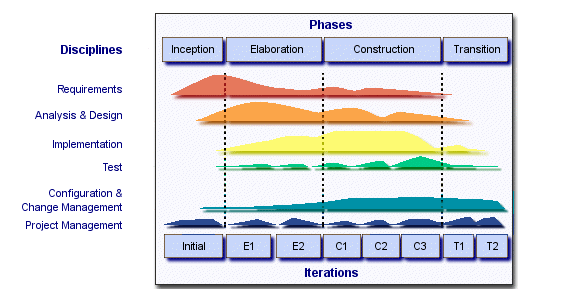
\includegraphics[scale=0.75]{images/upeduFases}
\caption{Fases de la metodología UPedu \cite{upedu}}
\end{center}
\end{figure}

En la figura anterior, se puede observar el esfuerzo necesario de cada disciplina en cada fase del proyecto

\paragraph{Fase de inicio}\mbox{}\\

En esta fase no se realiza ningún artefacto de tipo software, pues estos se deben tratar antes de comenzar con la implementación. Los objetivos fundamentales de esta fase son la definición del alcance del proyecto,  la determinación de los casos de uso críticos, la estimación del coste y la duración del proyecto, y la elaboración de una primera gestión de riesgos.

\paragraph{Fase de elaboración}\mbox{}\\

El objetivo fundamental de esta fase \cite{pgpup} es el de la elaboración del diseño y arquitectura del sistema informático. Similarmente, se realizará un análisis del dominio del sistema y se eliminarán los elementos de mayor riesgo para el desarrollo del proyecto.

Después de esta fase, se obtendrá una arquitectura, requisitos y planes de desarrollo estables. Similarmente, se habrán reducido los riesgos más destacables.

\paragraph{Fase de construcción}\mbox{}\\

Es sin ninguna duda la parte más larga del proyecto y es la primera que tendrá como output artefactos software utilizables.Se irá iterando y mejorando la calidad del producto software en cada ciclo.

La salida de esta fase \cite{pgpup} es software en estado beta.

\paragraph{Fase de transición}\mbox{}\\

Se deberá conseguir la aceptación por parte del usuario, indicando que cumple con la visión inicial del proyecto. Asímismo, se distribuirá el software.

\subsubsection{Calendario del proyecto}

Como se ha indicado en los apartados anteriores, este proyecto se ha dividido en las fases que el Proceso Unificado, en su variación UPedu\cite{upedu} establece. A continuación, se lista cada fase, el número de iteraciones y las horas de trabajo y duración estimadas. Estos cálculos son orientativos, las variaciones sobre los mismos están expuestas en el apartado correspondiente.

\begin{table}[H]
\centering
\begin{tabular}{|l|l|l|l|}
\hline
Nombre de la fase & Núm.. Iteraciones & Horas de trabajo & Duración estimada \\ \hline
Inicio            & 1                 & 10 horas/semana  & 6-7 semanas       \\ \hline
Elaboración       & 2                 & 10 horas/semana  & 10-11 semanas     \\ \hline
Construcción      & 2                 & 20 horas/semana  & 6-7 semanas       \\ \hline
Transición        & 1                 & 5 horas/semana   & 2-3 semanas       \\ \hline
\end{tabular}
\caption{Fases del proceso UPedu}
\end{table}

\paragraph{Fase de inicio}\mbox{}\\

Comienza el día 6 de Noviembre de 2017 y finaliza el 20 de Diciembre de 2017. Consta de una única iteración.

\begin{table}[H]
\centering
	\begin{tabular}{|l|l|l|l|}
    \hline
    Nombre de la tarea                           & Fecha de comienzo & Fecha de fin & Duración \\ \hline
    Estudio del sistema.                         & 06/11/2017        & 12/11/2017   & 7 días   \\ \hline
    Búsqueda de información.                     & 13/11/2017        & 15/11/2017   & 3 días   \\ \hline
    Resumen de la propuesta                      & 15/11/2017        & 18/11/2017   & 4 días   \\ \hline
    Estudio de aplicaciones móviles.             & 18/11/2017        & 22/11/2017   & 5 días   \\ \hline
    Elaboración de un prototipo inicial          & 23/11/2017        & 26/11/2017   & 4 días   \\ \hline
    Estudio de la posible tecnología a utilizar. & 27/11/2017        & 29/11/2017   & 3 días   \\ \hline
    Plan de Desarrollo de Software.              & 30/11/2017        & 04/12/2017   & 5 días   \\ \hline
    Elicitación de requisitos.                   & 05/12/2017        & 12/12/2017   & 8 días   \\ \hline
    Identificación de riesgos.                   & 13/12/2017        & 16/12/2017   & 4 días   \\ \hline
    Gestión de configuraciones.                  & 17/12/2017        & 20/12/2017   & 4 días   \\ \hline
    \end{tabular}
    \caption{Iteración 0. Fase de Inicio.}
\end{table}

\paragraph{Fase de elaboración}\mbox{}\\

Comienza el día 20 de Diciembre de 2017 y finaliza el 1 de Marzo de 2018. Consta de dos iteraciones.

\begin{table}[H]
\centering
\begin{tabular}{|l|l|l|l|}
\hline
Nombre de la tarea          & Fecha de comienzo & Fecha de fin & Duración \\ \hline
Revisión de requisitos      & 21/12/2017        & 23/12/2017   & 3 días   \\ \hline
Diagrama de casos de uso    & 24/12/2017        & 27/12/2017   & 4 días   \\ \hline
Realización de casos de uso & 28/12/2017        & 18/01/2018   & 22 días  \\ \hline
Diagramas de secuencia      & 19/01/2018        & 28/01/2018   & 10 días  \\ \hline
Diseño de la Base de Datos  & 29/01/2018        & 04/02/2018   & 7 días   \\ \hline
Plan inicial de pruebas     & 05/02/2018        & 10/02/2018   & 6 días   \\ \hline
Arquitectura del sistema    & 11/02/2018        & 18/02/2018   & 8 días   \\ \hline
\end{tabular}
\caption{Iteración 1. Fase de elaboración.}
\end{table}

En la figura anterior, he puesto una duración de 22 días a la realización de casos de uso porque en ese período lo dedicaré a la preparación de los exámenes del primer cuatrimestre y únicamente dedicaré los tiempos libres a la realización del Trabajo Fin de Grado. 

\begin{table}[H]
\centering
\begin{tabular}{|l|l|l|l|}
\hline
Nombre de la tarea                           & Fecha de comienzo & Fecha de fin & Duración \\ \hline
Actualización de casos de uso                & 18/02/2018        & 20/02/2018   & 3 días   \\ \hline
Actualización de diagramas de secuencia      & 21/02/2018        & 23/02/2018   & 3 días   \\ \hline
Actualización del diseño de la Base de Datos & 24/02/2018        & 25/02/2018   & 2 días   \\ \hline
Actualización de Plan inicial de pruebas     & 27/11/2017        & 28/11/2017   & 2 días   \\ \hline
Actualización de la arquitectura del sistema & 28/02/2018        & 01/03/2018   & 2 días   \\ \hline
\end{tabular}
\caption{Iteración 2.Fase de elaboración.}
\end{table}

\paragraph{Fase de construcción}\mbox{}\\

Comienza el día 1 de Marzo de 2018 y finaliza el 16 de Abril de 2018.

\begin{table}[H]
\centering
\begin{tabular}{|l|l|l|l|}
\hline
Nombre de la tarea             & Fecha de comienzo & Fecha de fin & Duración \\ \hline
Implementación del sistema     & 01/03/2018        & 01/04/2018   & 32 días  \\ \hline
Realización de casos de prueba & 01/03/2018        & 01/04/2018   & 32 días  \\ \hline
\end{tabular}
\caption{Iteración 3. Fase de construcción.}
\end{table}

\begin{table}[H]
\centering
\begin{tabular}{|l|l|l|l|}
\hline
Nombre de la tarea                & Fecha de comienzo & Fecha de fin & Duración \\ \hline
Implementación del sistema        & 01/04/2018        & 16/04/2018   & 16 días  \\ \hline
Elaboración del manual de usuario & 17/04/2018        & 24/04/2018   & 8 días   \\ \hline
Realización de casos de prueba    & 01/04/2018        & 16/04/2018   & 16 días  \\ \hline
\end{tabular}
\caption{Iteración 4. Fase de construcción.}
\end{table}

\paragraph{Fase de transición}\mbox{}\\

Comienza el día 16 de Abril de 2018 y finaliza el 30 de Abril de 2018.

\begin{table}[H]
\centering
\begin{tabular}{|l|l|l|l|}
\hline
Nombre de la tarea              & Fecha de comienzo & Fecha de fin & Duración \\ \hline
Revisión de documentación       & 16/04/2018        & 23/04/2018   & 8 días   \\ \hline
Revisión de artefactos software & 23/04/2018        & 30/04/2018   & 8 días   \\ \hline
\end{tabular}
\caption{Iteración 5. Fase de transición.}
\end{table}

\subsection{Relación de artefactos no software}

Los distintos entregables a realizar son los siguientes. En todo caso, siempre se considerará como definitiva la versión final de los documentos entregados.
\paragraph{Fase de inicio\\}
\begin{itemize}
\item Plan de Desarrollo de Software.
\item Versión inicial del Plan de Gestión de Riesgos.
\end{itemize}
\paragraph{Fase de elaboración\\}
\begin{itemize}
\item Documento de requisitos \textit{software}.
\item Versión inicial de los Casos de Uso.
\item Diagramas de secuencia.
\item Arquitectura del sistema.
\item Diseño de la Base de Datos.
\item Elaboración de prototipos.
\end{itemize}

\paragraph{Fase de construcción\\}
\begin{itemize}
\item Versión inicial del manual de usuario.
\item Documento de casos de prueba.
\item Documento de resultados de las pruebas.
\end{itemize}

\paragraph{Fase de transición\\}
\begin{itemize}
\item Versión final del manual de usuario.
\end{itemize}

\subsection{Control y seguimiento del proyecto.}

Se hará un control y seguimiento del proyecto en todo momento, utilizando la herramienta Zoho Projects \footnote{\url{https://projects.zoho.com/}}, tal y como se ha expuesto en el apartado "Herramientas utilizadas".

El control y seguimiento del proyecto resulta ser una tarea fundamental para asegurar el buen progreso del proyecto y asegurar el cumplimiento de los objetivos marcados, en especial en cuanto al cumplimiento de los hitos establecidos, ya que el gestor del proyecto podrá observar las distintas variaciones de tiempo programadas versus reales para así poder reaccionar y poder tomar las medidas que sean precisas para ajustarse al cronograma del proyecto.

\subsection{Gestión de riesgos.}

Se identifican los siguientes riesgos:

\begin{risk}
  \addheading{R0}{Falta de experiencia del alumno}
  \addrow{Descripción}{El alumno ha realizado prácticas en Android, pero puede encontrarse en momentos en los que requiera experiencia adicional.}
  \addrow{Consecuencia}{Ralentización del trabajo.}
  \addrow{Probabilidad}{Media.}
  \addrow{Impacto}{Bajo.}
  \addrow{Estrategia}{Reservar el riesgo}
  \addrow{Plan de acción}{Buscar información y ayuda, ya sea preguntando a la tutora del trabajo o utilizando otros medios.}
  \addrow{Plan de contingencia}{Revisión de conocimientos existentes.}
\end{risk}

\begin{risk}
  \addheading{R1}{Retraso en la planificación}
  \addrow{Descripción}{Debido a errores en la estimación, la planificación no se ajusta a la realidad y se producen demoras en las fechas de entrega.}
  \addrow{Consecuencia}{Retraso en la entrega de los artefactos.}
  \addrow{Probabilidad}{Alta }
  \addrow{Impacto}{Crítico}
  \addrow{Estrategia}{Reservar el riesgo}
  \addrow{Plan de acción}{Realizar una nueva planificación más realista. }
  \addrow{Plan de contingencia}{Realizar revisiones periódicas del calendario de planificación.}
\end{risk}

\begin{risk}
  \addheading{R2}{Adelantos en la planificación}
  \addrow{Descripción}{Debido a errores en la estimación, la planificación no se ajusta a la realidad y se producen adelantos en las fechas de entrega.}
  \addrow{Consecuencia}{Modificación de toda la planificación.}
  \addrow{Probabilidad}{Alta }
  \addrow{Impacto}{Crítico}
  \addrow{Estrategia}{Reservar el riesgo}
  \addrow{Plan de acción}{Realizar una nueva planificación más realista. }
  \addrow{Plan de contingencia}{Realizar revisiones periódicas del calendario de planificación.}
\end{risk}

\begin{risk}
  \addheading{R3}{Falta de experiencia en grandes proyectos.}
  \addrow{Descripción}{El equipo no cuenta con experiencia propia de proyectos de gran extensión que le permita calcular mejor las estimaciones, así como realizar el proyecto con mayor celeridad.}
  \addrow{Consecuencia}{Peor organización y estimaciones. Grandes picos de trabajo.}
  \addrow{Probabilidad}{Alta }
  \addrow{Impacto}{Alto. }
  \addrow{Estrategia}{Reducción del riesgo.}
  \addrow{Plan de acción}{Realizar una nueva planificación. }
  \addrow{Plan de contingencia}{Realizar revisiones periódicas del calendario de planificación.}
\end{risk}

\begin{risk}
  \addheading{R4}{Falta de disponibilidad}
  \addrow{Descripción}{El alumno no puede continuar con el trabajo por falta de disponibilidad.}
  \addrow{Consecuencia}{Dependerá del tiempo en el que esté no disponible y las holguras en la planificación. Si es muy largo, puede suponer la no entrega del trabajo a tiempo.}
  \addrow{Probabilidad}{Baja.}
  \addrow{Impacto}{Crítico. }
  \addrow{Estrategia}{Reservar del riesgo.}
  \addrow{Plan de acción}{Realizar una nueva planificación basándose en las nuevas fechas \\de disponibilidad.}
  \addrow{Plan de contingencia}{Monitorizar la disponibilidad del alumno.}
\end{risk}

\begin{risk}
  \addheading{R5}{Pérdida de datos}
  \addrow{Descripción}{Por cualquier motivo, se pierde total o parcialmente cualquiera de los artefactos ya realizados o en proceso de realización.}
  \addrow{Consecuencia}{Ralentización muy alta del trabajo. Repetición de los artefactos perdidos. }
  \addrow{Probabilidad}{Bajo.}
  \addrow{Impacto}{Crítico. }
  \addrow{Estrategia}{Evitación del riesgo.}
  \addrow{Plan de acción}{No se aplica}
  \addrow{Plan de contingencia}{Realización de copias de seguridad y uso de un sistema de control de versiones (ver apartado gestión de configuraciones)}
\end{risk}

\begin{risk}
  \addheading{R6}{Falta de medios software de desarrollo}
  \addrow{Descripción}{Las herramientas designadas para desarrollar el proyecto fallan, desaparecen o dejan de estar disponibles.}
  \addrow{Consecuencia}{Ralentización muy alta del trabajo. Repetición de los artefactos perdidos. }
  \addrow{Probabilidad}{Bajo.}
  \addrow{Impacto}{Crítico. }
  \addrow{Estrategia}{Evitación del riesgo.}
  \addrow{Plan de acción}{No se aplica}
  \addrow{Plan de contingencia}{Utilización de herramientas profesionales, aplicación de las últimas actualizaciones.}
\end{risk}

\begin{risk}
  \addheading{R7}{Falta de medios hardware de desarrollo}
  \addrow{Descripción}{Las herramientas designadas para desarrollar el proyecto fallan o dejan de estar disponibles.}
  \addrow{Consecuencia}{Adquisición de nuevos materiales.}
  \addrow{Probabilidad}{Bajo.}
  \addrow{Impacto}{Alto. }
  \addrow{Estrategia}{Evitación del riesgo.}
  \addrow{Plan de acción}{No se aplica}
  \addrow{Plan de contingencia}{Realización de copias de seguridad de los artefactos, para evitar su pérdida en caso de ocurrir este riesgo.}
\end{risk}

\begin{risk}
  \addheading{R8}{Diseño pobre o incorrecto.} 
  \addrow{Descripción}{El diseño realizado del sistema es pobre o incorrecto.}
  \addrow{Consecuencia}{Ralentización del trabajo.}
  \addrow{Probabilidad}{Medio.}
  \addrow{Impacto}{Crítico. }
  \addrow{Estrategia}{Reducción del riesgo.}
  \addrow{Plan de acción}{Rediseñar la arquitectura del sistema.}
  \addrow{Plan de contingencia}{Realizar revisiones con el cliente y realizar pruebas sobre el modelo diseñado.}
\end{risk}

\subsection{Gestión de configuraciones.}

Hoy en día, la mayoría de los servicios públicos que ofrecen alojamiento de repositorios Git permiten realizar una buena gestión de configuraciones. Esto es debido a que cada cambio que se hace sobre el código fuente (\textit{commit}) viene asociado a informaciones sobre qué se ha cambiado, quién lo ha cambiado, cuándo lo ha cambiado, etcétera. Además, las ramas o \textit{branches}, aquellos lugares donde van dirigidos los cambios, permiten imponer bloqueos sobre escritura a ciertos usuarios, con el fin de proteger los artefactos que estuvieran en la misma.

Por otro lado, estos servicios también pueden ser utilizados para la gestión de \textit{releases}. Esto se puede llevar a cabo mediante la creación de una rama específica para ese propósito o, directamente, y si se permite, mediante el apartado correspondiente desde el sitio web.

En el caso de este proyecto se han utilizado dos repositorios privados en GitHub\footnote{\url{https://github.com/}}, en uno de ellos se tratará el desarrollo de esta memoria y en otro, el del código del sistema informático que se desea construir.

\subsection{Costes.}

Para el cálculo de los costes de los recursos, debemos diferenciar entre los costes propios de los humanos, frente a los informáticos, que incluyen aquellos de tipo \textit{hardware} y de tipo \textit{software}

Para el caso de los primeros, los costes de los recursos humanos, debemos ver el listado de roles que se van a practicar a lo largo del proyecto:

\begin{table}[]
\label{my-label}
\begin{tabular}{|l|l|l|l|l|}
\hline
Rol                & Salario medio & \euro/Hora   & Horas estimadas & Coste total \\ \hline
Analista           & 26.307 \euro      & 109,61 \euro & 12              & 1           \\ \hline
Desarrollador      & 17.411 \euro      & 72,55 \euro  & 1               & 1           \\ \hline
Gestor de proyecto & 26.307 \euro      & 109,61 \euro & 1               & 1           \\ \hline
Diseñador          & 26.307 \euro      & 109,61 \euro & 1               & 0           \\ \hline
\end{tabular}
\caption{Costes de los Recursos Humanos}
\end{table}

Los datos de la tabla anterior han sido calculados basándose en los datos de \cite{indeedanalista} para el salario bruto anual de un Analista de Software (26.307 \euro) y los de \cite{indeedjunior} (17.411 \euro) para el de Programador Junior. Se ha dividido la cantidad anterior en doce pagas y veinte días de trabajo por mes.

Por otra parte, los costes informáticos de \textit{hardware} no resultan de especial interés, pues son dispositivos con una cierta antigüedad y el coste amortizado será, por tanto, mínimo. 

Finalmente, en el software sí encontramos ciertos costes. Se ha de tener presente que estos son cálculos que sí se aplicarían en un proyecto en el que no se pudieran utilizar licencias gratuitas para estudiantes.

\begin{table}[]
\centering

\begin{tabular}{|l|l|l|}
\hline
Servicio         & Coste mensual & Coste total \\ \hline
GitHub Developer & 5.90 \euro        & 47.2\euro          \\ \hline
Firebase         & 21 \euro      & 168\euro           \\ \hline
\end{tabular}
\caption{Costes de software}
\end{table}

Coste total de software: 215,20\euro

Los datos anteriores se han calculado basándose en los datos públicos de las herramientas, convertido a euros según la tasa de cambio del 28 de Noviembre de 2017, para un período de 8 meses (Noviembre-Junio).

El resto de \textit{software} utilizado es de licencia gratuita.


\begin{usecase}
  \addheading{CU001}{System user} 
  \addrow{Actor}{T}
  \addrow{Precondition}{The system, shows, in the form part of an object type, the number indication.}
  \addrow{Postcondition}{A disconnected number indicating the type of `other constructed object'.}
  \addmulrow{Main path (M)}{
  							\item User selects \ldots
                            \item System demands \ldots
  }
\end{usecase}


\subsection{Desviaciones sobre el calendario planificado}
A realizar cuando sea preciso.
\section{Requisitos}
\subsection{Requisitos funcionales}
\begin{req}
	\addheading{RF0}{Sesiones}
	\addrow{Descripción}{El sistema permitirá iniciar sesión}
\end{req} \\
 
\begin{req}
	\addheading{RF1}{Registro de usuarios}
	\addrow{Descripción}{El sistema permitirá registrar usuarios}
\end{req}\\

\begin{req}
	\addheading{RF2}{Configuración del usuario}
	\addrow{Descripción}{El sistema permitirá editar la configuración del usuario}
\end{req}\\

\begin{req}
	\addheading{RF3}{Identificación del tipo de jugador}
	\addrow{Descripción}{El sistema identificará el tipo de jugador.}
\end{req}\\

\begin{req}
	\addheading{RF3}{Ranking de usuarios}
	\addrow{Descripción}{El sistema permitirá ver el ranking de usuarios}
\end{req}\\

	

\subsection{Requisitos no funcionales}


\chapter{Referencias}
\begin{thebibliography}{a} 

\bibitem{cristinatfg} \textsc{Cristina Martínez Martínez} \textit{TFG “Estudio de gamificación en una empresa para mejorar la fidelización de los clientes”}. Curso 2016-2017. Grado en Organización Industrial. Universidad de Valladolid. 

\bibitem{anatfg} \textsc{Ana Ruiz Caballero} \textit{TFG "Estudio de la gamificación de una empresa para incentivar la motivación."}. Curso 2015-2016. Grado en Organización Industrial. Universidad de Valladolid. 

\bibitem{iebschoolGami} \textsc{Marc Rodríguez. IEBS Comunidad} \textit{La gamificación como fenómeno social y herramienta global}, Fecha de última visita: 6 de Noviembre de 2017 \url{http://comunidad.iebschool.com/pedrolopezugarte/2015/11/20/la-gamificacion-como-fenomeno-social-y-herramienta-global/}.  

\bibitem{bbvag} \textsc{Alejandro. Omnium Games.} \textit{BBVA Game: El mayor caso de éxito de la gamificación en España.}, Fecha de última visita: 21 de Noviembre de 2017 \url{http://omniumgames.com/bbva-game-el-mayor-caso-de-exito-de-la-gamificacion-en-espana/}.  

\bibitem{iebsctj} \textsc{Ferran Altarriba Bertran. IEBS School} \textit{Tipos de jugadores en Gamification: teoría Bartle}. Fecha de última visita: 6 de Noviembre de 2017, \url{http://www.iebschool.com/blog/tipos-jugadores-gamification-2-innovacion/}.  

\bibitem{mcdo} \textsc{McDonalds},\textit{Aplicación móvil McDonalds para Android} \url{https://play.google.com/store/apps/details?id=com.mcdonalds.android}


\bibitem{burgerk} \textsc{Burger King},\textit{Aplicación móvil Burger King para Android} \url{https://play.google.com/store/apps/details?id=es.burgerking.android}

\bibitem{kfcapp} \textsc{KFC},\textit{Aplicación móvil KFC para Android} \url{https://play.google.com/store/apps/details?id=es.kfc.spain}

\bibitem{vipsapp} \textsc{VIPS},\textit{Aplicación móvil VIPS para Android} \url{https://play.google.com/store/apps/details?id=com.clubvips.app}

\bibitem{pansapp} \textsc{Pans \& Company},\textit{Aplicación móvil Pans \& Company para Android} \url{https://play.google.com/store/apps/details?id=es.eatout.panscompany}

\bibitem{fostersh} \textsc{Foster's Hollywood},\textit{Aplicación móvil Foster's Hollywood para Android} \url{https://play.google.com/store/apps/details?id=com.zena.Fosters}

\bibitem{androidversiondist} \textsc{Android Developers Official Website},\textit{Dashboards. Platform Versions.} Fecha de última visita: 25 de Noviembre de 2017 \url{https://developer.android.com/about/dashboards/index.html}

\bibitem{pgpup} \textsc{Pablo de la Fuente Redondo. Departamento de Informática de la UVa}, \textit{Apuntes de la asignatura Planificación y Gestión de Proyectos. Curso 2017-2018. Proceso Unificado}

\bibitem{upedu} \textsc{Unified Process for Education. Universidad Politécnica de Montreal}. Fecha de última visita: 25/11/2017\url{http://www.upedu.org/process/workers/wk_implm.htm}

\bibitem{indeedanalista} \textsc{Indeed}. Salario medio de un Analista Programador en España. Fecha de última visita: 28/11/2017 \url{https://www.indeed.es/salaries/Analista-programador/a-Salaries}

\bibitem{indeedjunior} \textsc{Indeed}. Salario medio de un Programador Junior en España. Fecha de última visita: 28/11/2017 \url{https://www.indeed.es/salaries/Programador/a-junior-Salaries}



\end{thebibliography}

\chapter{Anexos}



\end{document}